\documentclass[xcolor=dvipsnames, 12pt, handout]{beamer}
\useoutertheme{infolines} 
%\definecolor{grayish}{RGB}{147,162,153}
\usecolortheme[named=gray]{structure} 
\usetheme[height=7mm]{Rochester}

\usepackage{graphicx}

\usepackage{AMMALanguages}
\usepackage{hyperref}
\usepackage{tikz}
\usetikzlibrary{positioning}
\usetikzlibrary{arrows,shapes}

%\setbeameroption{show notes}
%\setbeameroption{show only notes}
\setbeamertemplate{note page}[plain]

\usepackage[utf8]{inputenc}
\usepackage[T1]{fontenc}

\usepackage{listings}

\newcommand\blfootnote[1]{%
  \begingroup
  \renewcommand\thefootnote{}\footnote{#1}%
  \addtocounter{footnote}{-1}%
  \endgroup
}

\AtBeginSection{\frame{\sectionpage}}

\title[SyVOLT]{SyVOLT: Full Model Transformation Verification Using Contracts}
%\title{Full Verification of Model Transformation Contracts for Declarative ATL}
\author[Lucio et al.]{Levi L\'{u}cio, \textbf{Bentley James Oakes}, Claudio Gomes, Gehan Selim, Juergen Dingel, James R. Cordy, Hans Vangheluwe}
%\subtitle{}
%\logo{}
\institute[]{McGill University, Canada\\University of Antwerp, Belgium\\Queen's University, Canada}
%\date{}
%\subject{}
%\setbeamercovered{transparent}
%\setbeamertemplate{navigation symbols}{}

% logo of my university
%\titlegraphic{\vspace{-0.5cm}\includegraphics[width=3cm]{figures/mcgill}\hspace*{4.75cm}~%
%   \includegraphics[width=4cm]{figures/big}
%}

\begin{document}
\maketitle

%\section{Intro}

\begin{frame}{Motivation and Overview}
\begin{itemize}[<+->]
\item Model transformations are at the heart of model-driven engineering
\item Want to verify correctness for transformation specifications
\begin{itemize}[<+->]
\item Verify visual contracts
\item Identify combinations of rules where contracts hold or not
\end{itemize}
\item Objective: Verification for all input models
\begin{itemize}
\item Input independence
\end{itemize}
\end{itemize}
\end{frame}


%\section{Families-To-Persons Transformation}




\begin{frame}{DSLTrans Transformation}

\begin{itemize}[<+->]
\item Visual language for model transformations

\item Graph-based, rule-based
\item Out-place so no rewriting performed
\begin{itemize}
\item Suited for `translation' transformations
\end{itemize}
\item All its computations are terminating and confluent
\item Unbounded loops during execution are not allowed

\item Rules are grouped in sequential layers
\end{itemize}

\blfootnote{Selim, Gehan et al. "Model transformations for migrating legacy deployment models in the automotive industry." Software and Systems Modeling 14, no. 1 (2013): 365-381.}

\end{frame}


\begin{frame}{Transformation Metamodels}

\begin{center}
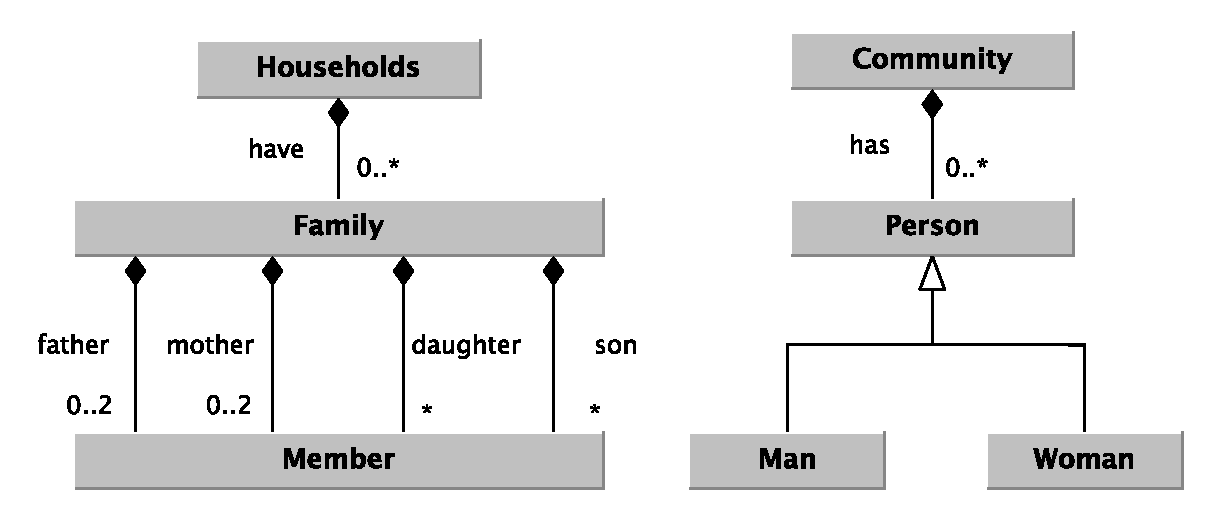
\includegraphics[width=0.8\textwidth]{figures/Metamodels_F2P}
\end{center}
\begin{itemize}
\item Transform \textit{Members} to \textit{Men} and \textit{Women}
\end{itemize}
\end{frame}


\begin{frame}{DSLTrans}
\begin{center}
\includegraphics[width=\textwidth]{figures/Rules}
\end{center}
\pause
\begin{itemize}[<+->]
\item Rules arranged in layers
\item Match graph on top of rules
\item Apply graph on bottom
\begin{itemize}
\item Produced when match graph is found
\end{itemize}
\end{itemize}
\end{frame}




\begin{frame}{Contracts}
\begin{center}
\includegraphics[width=0.40\textwidth]{figures/fourMembersProp}
\end{center}
\pause
\begin{itemize}[<+->]
\item Pre- / post- visual contracts
\item If blue graph is found in input model, then red graph is found in output model
\item Objective: Prove for all input models/transformation executions - input independence
\item \textit{A family with a father, mother, son, daughter
should always produce two males and two females in the
target community}
\end{itemize}
\end{frame}


\begin{frame}{Contracts}
\begin{center}
\includegraphics[width=0.45\textwidth]{figures/motherFatherProp}
\end{center}
\pause
\begin{itemize}[<+->]
\item Reasoning about attributes of elements
\item \textit{Is the full name of the produced Person correctly created from the last name of the Family and the first name of the Member?}
\end{itemize}
\end{frame}

\begin{frame}{Contracts}
\begin{center}
\includegraphics[width=0.5\textwidth]{figures/daughterMotherProp}
\end{center}
\begin{itemize}[<+->]
\item A contract that will not hold
\item \textit{A family with a mother and a daughter will always produce a community with a man}
\end{itemize}
\end{frame}


\begin{frame}{SyVOLT Tool}
\begin{itemize}[<+->]
\item Tool to prove visual contracts on DSLTrans transformations
\item All possible executions of the transformation are symbolically constructed
\begin{itemize}[<+->]
\item Built as sets of rules called path conditions
\begin{itemize}
\item No rules execute, only rule 1 executes, rule 1 and rule 2 both execute
\item Rule dependencies/combinations resolved
\end{itemize}
\item Final set of path conditions represents all possible transformation executions
\end{itemize}
\item A contract holds for a transformation if it holds for all generated path conditions
\end{itemize}
\blfootnote{L. Lúcio, B. Oakes, and H. Vangheluwe. A technique for symbolically verifying properties of graph-based model transformations. Technical report, Technical Report SOCS-TR-2014.1, McGill U, 2014.}
\end{frame}

\begin{frame}{Other Work at MODELS 2015}
\small
\begin{itemize}[<+->]
\item Poster available for SyVOLT tool
\item Fully Verifying Transformation Contracts for Declarative ATL (MODELS)\\
Bentley James Oakes, Javier Troya, Levi Lucio, and Manuel Wimmer\\
(McGill University, Canada; Vienna University of Technology, Austria)\\
Thursday at 3:30 PM
\item  Finding and fixing bugs in model transformations with formal verification: An experience report (AMT)\\
Gehan M. K. Selim, James R. Cordy, Juergen Dingel, Levi Lucio and Bentley James Oakes\\
(Queen's University, Canada; McGill University, Canada) 
%\item Model transformations for migrating legacy deployment models in the automotive industry.\\
%Selim, Gehan et al. \\
 %Software and Systems Modeling 14
\end{itemize}
\end{frame}


%\section{Mapping ATL to DSLTrans}



%\section{Generating Path Conditions}



%\section{Results}

%\section{Conclusion and Thanks}

\begin{frame}{Conclusion}
\begin{itemize}[<+->]
\item Can verify visual contracts on DSLTrans transformations in feasible time
\item Contracts verified on all transformation executions
\item Eclipse plugin to build transformation and contracts
\item Future work is to focus on contract-driven development of model transformations
\end{itemize}
\pause
\begin{itemize}
\item Thank you for your time!
\end{itemize}
\begin{center}
\textbf{SyVOLT: Full Model Transformation Verification Using Contracts}\\
\textbf{Levi L\'{u}cio, \textbf{Bentley James Oakes}, Claudio Gomes, Gehan Selim, Juergen Dingel, James R. Cordy, Hans Vangheluwe}\\
\url{http://msdl.cs.mcgill.ca/people/levi/files/MODELS2015}

\end{center}
\end{frame}


\end{document}
